\documentclass[a4paper,12pt]{book}
\usepackage[utf8]{inputenc}
\usepackage{graphicx}
\usepackage[english]{babel}
\usepackage{amsmath}
\usepackage{tabularx}
\usepackage{graphicx}
\usepackage{pbox}
\usepackage{framed}
\usepackage{units}
\usepackage[table, dvipsnames]{xcolor}
\usepackage[hidelinks]{hyperref}
\usepackage{tikz}
\usepackage{placeins}
\usepackage{pdflscape}
\usepackage{makeidx}
\usepackage{subfig}
\usepackage{amsmath}
\usepackage{amsfonts}
\usepackage{amssymb}
\usepackage{rotating}
\usepackage[export]{adjustbox}
\usepackage{tcolorbox}
\usepackage{multicol}
\usepackage[T1]{fontenc}
\usepackage[utf8]{inputenc}
\usepackage{titlesec}
\usepackage{etoolbox}
\usepackage{marginnote}
\usepackage{url}
\usepackage{float}
\usepackage[binary-units]{siunitx}
\usepackage{xlop}
\usepackage[chapter]{minted}
\usepackage{karnaughmap}
\usepackage{circuitikz}
\usepackage{natbib}
\usepackage [autostyle, english = british]{csquotes}
%\usepackage{gnuplot}


\newcolumntype{M}[1]{>{\centering\arraybackslash}m{#1}}
\newcolumntype{T}[1]{>{\ttfamily\centering\arraybackslash}m{#1}}
\newcolumntype{R}[1]{>{\flushright\arraybackslash}m{#1}}
\newcolumntype{L}[1]{>{\centering\flushleft\arraybackslash}m{#1}}
\newcolumntype{C}[1]{>{\centering\arraybackslash}m{#1}}

%%% Biblography Commands

\setlength{\bibsep}{3mm}
\setlength{\bibhang}{5em}
\bibliographystyle{agsm}
\setcitestyle{authoryear,round}


%%% Chapter Statment 

\newenvironment{statement}
{
	
	\begin{center}
		\begin{minipage}[c]{0.8\textwidth}
			\it
				
			}
			{		
			\it
		\end{minipage}
	\end{center}
}

\renewcommand \thepart {\arabic{part}}
\renewcommand\thechapter{\thepart.\arabic{chapter}}

\makeatletter
\@addtoreset{chapter}{part}
\makeatother


\setkarnaughmap[omitzeros=false,omitidx=true]
\DeclareSIUnit{\year}{yrs}



\makeindex
\makeglossary

\begin{document}
\title{A Level Computing}
\date{\today}

\newcommand\bonus{\textcolor{Black!80}{\textbf{BONUS: }}}
\newcommand\bigo[1]{\mathcal{O}(#1)}
\newcommand\bigO[1]{$\bigo{#1}$}
\newcommand{\true}{\mintinline{c}{true} }
\newcommand{\false}{\mintinline{c}{false} }
\newcommand{\code}[2][c]{\mintinline{#1}{#2}}
\newcommand{\RTL}[1]{\mintinline[escapeinside=||]{hs}{#1}}
\newcommand{\ARM}[1]{\mintinline[escapeinside=||]{arm}{#1}}
\newcommand{\LMC}[1]{\texttt{#1}}
\newminted{c}{}
\newmintinline{c}{}

\usemintedstyle{bw}
\renewcommand{\listingscaption}{Snippet}
\maketitle
\frontmatter
\tableofcontents

\mainmatter

\part{Binary Manipulation}
	\chapter{What is Binary?}
	\section{Introduction}
	In school, you learnt to count and do arithmetic in \textit{decimal}. Just as you have 10 fingers, there are 10 decimal digits $0,1,2, ..., 9$. Decimal digits are joined together to form longer decimal numbers. Each column of a decimal number has ten times the weight of the previous column. From right to left, the column weights are $1, 10, 100, 1000$ and so on. In general we can say that the $n^{th}$ has a value of $10 ^{(n - 1)}$.

	\begin{equation}
	9742_{10} = 9 \times 10^3 + 7 \times 10^2 + 4 \times 10^1 + 2 \times 10^0
	\end{equation}

	We can generalise this and say for a number $n$ in base $b$ which has digits $n_1, n_2, n_3, \dots n_{m-1}, n_m$ has a value of $N$ which is given by Equation \ref{equ:anynumber}

	\begin{equation}
		N = \sum_{i=0}^{i=m} n_i \times b^i
		\label{equ:anynumber}
	\end{equation}

	Computers are made up of lots of little tiny electrical switches that have two states: one or off. We represent this using a binary number system.	We use the digits 0 or 1 to mean off and on respectively  Each digit is known as a bit and is a fundamental unit of information. We find that using a $n$-digit binary number we can represent $2^n$ different values. Table \ref{tab:BinandDec} shows this in action.
	\begin{table}[h]
		\begin{center}
		\begin{tabular}{M{0.15\linewidth}M{0.15\linewidth}M{0.15\linewidth}M{0.15\linewidth}M{0.15\linewidth}}
				\multicolumn{4}{c}{Binary Numbers} & Decimal Equivalent\\

				1-Bit	& 2-Bit	& 3-Bit	& 4-Bit	&		\\
				\hline
				\hline
				0		& 00	& 000	& 0000	& 0		\\
				1		& 01	& 001	& 0001	& 1		\\
						& 10	& 010	& 0010	& 2		\\
						& 11	& 011	& 0011	& 3		\\
						& 		& 100	& 0100	& 4		\\
						& 		& 101	& 0101	& 5		\\
						& 		& 110	& 0110	& 6		\\
						& 		& 111	& 0111	& 7		\\
						& 		& 		& 1000	& 8		\\
						& 		& 		& 1001	& 9		\\
						& 		& 		& 1010	& 10	\\
						& 		& 		& 1011	& 11	\\
						& 		& 		& 1100	& 12	\\
						& 		& 		& 1101	& 13	\\
						& 		& 		& 1110	& 14	\\
						& 		& 		& 1111	& 15	\\
			\end{tabular}
			\caption{\label{tab:BinandDec} Binary Numbers and their Decimal Equivalent}
		\end{center}
	\end{table}
	\subsection{Grouping Bits}
		A group of eight bits is called a \textit{byte}. One byte can take $2^8 = 256$ possible values. Generally we measure the size of computer storage / memory in bytes rather than bits. We can also store data in a nibble, which is 4 bits. This gives you $2^4 = 16$ possible values, or one hexadecimal digit. Often when dealing with binary outputs we represent each byte as two hexadecimal digits. So \texttt{11010010} would be represented as \texttt{D2}.

		Microprocessors handle data in chunks known as \textit{words}. The size of the word depends on the architecture used. Most computers these days use 64-bit computers, so they have 64-bit words. However, Arduino's use 8 bit words.

	\subsection{File Sizes}
		A video file might contain 1,039,297,516 bytes, this is clearly to big to be practical. There are two different schemes for simplifying bytes, one uses powers of 10 and the other powers of 2. The decimal prefixes follow the standard SI units: kilo, mega, giga etc. The binary prefixes follow the following pattern:
			\begin{description}
				\item[kibi] \si{\kibi} - \si[prefixes-as-symbols=false]{\kibi}
				\item[mebi] \si{\mebi} - \si[prefixes-as-symbols=false]{\mebi}
				\item[gibi] \si{\gibi} - \si[prefixes-as-symbols=false]{\gibi}
				\item[tebi] \si{\tebi} - \si[prefixes-as-symbols=false]{\tebi}
			\end{description}
		So our video file from earlier is \SI{1.03929}{\giga\byte} or \SI{991.15}{\mebi\byte}. The difference between a \si{\kibi\byte} and \si{\kilo\byte} is why when you install a \SI{1}{\tera\byte} hard drive it appears as \SI{931}{\gibi\byte}.
\section{Exercises}
\subsection{Exam Style Questions}
\begin{enumerate}
	\item A flying saucer crashes into a cornfield. The investigators inspect the wreckage and find an engineering manual contain an equation in the Martian number system: $325 + 42 = 411$. If this equation is correct, how many fingers would you expect Martians to have?
	\item Alice and Bob are having an argument. Bob says \enquote{All integers greater than zero and exactly divisible by six have exactly two 1's in their binary representation}. Alice disagrees, she says: \enquote{No, but all such numbers have an even number of 1's in their representation.} Do you agree with Alice, Bob, both or neither. Explain.
\end{enumerate}
\subsection{Programming Challenges}
\begin{enumerate}
	\item Write a program in Python to convert numbers from binary to decimal. The user should type in an unsigned binary number. The program should printout the decimal equivalent

	\bonus Change your program from an arbitrary base $b_1$ to another base $b_2$ as specified by the user. Support bases up to 16, using the letters of the alphabet for digits greater than 9.
\end{enumerate}
	
	% !TeX root = ../main.tex

\chapter{Boolean Logic}
	\section{Boolean Algebra}
		\index{Boolean Algebra}
		Boolean Algebra was developed by an English Mathematician who specialised in the field of Logic. In 1854 he published \textit{ \enquote{An Investigation of Laws and Thought} \citep{Boole54}} which layed out the framework. Formally, boolean algebra is defined as of a set of elements, $E$, a set of functions, $F$ and and a set of basic axioms that define the properties of $E$ and $F$. In Boolean Algebra the set of elements are variables and constants that can either have a value of \true or \false. In addition there are only three operations or functions that are permitted. The first of these is the logical OR \index{OR!Logical}, represented by a plus (e.g. $A + B$ \footnote{Some texts will also use $\cup$ or $\vee$}). The Logical OR operation returns \true if either of the values is also \true. For example $A + B$ will return \true if either $A$ or $B$ is \true. Next we have the logical AND \index{AND!Logical}, represented by a dot (e.g. $A \cdot B$ \footnote{Some texts will also use $\times$, $\cap$ or $\wedge$. Also note that like in Maths, you can write $A \cdot B$ as $AB$.}). The Logical AND operation returns \true if all of the values are true will return The third operation is that of negation or complementation, we denote a variable having been negated with a bar (e.g. $\bar{A}$) \footnote{Some texts will also use !, ~, ¬, '} \index{NOT!Logical}. 
		
		
		We can combine these operations together to make new operations. As example lets take the exclusive-OR, or XOR function \index{XOR!Logical}. We define $A \oplus B$ \footnote{Some texts will also use $\veebar$} as returning \true when one, and only one, of its inputs are \true. The XOR operation can also be represented as 
		
		$$A \oplus B = A\cdot \bar{B} + \bar{A}\cdot B$$
		
		As mentioned in the previous chapter bits are the fundamental unit of the computer. This stream of 0's and 1's are what allow you to watch videos online, post to social media and order 200 rubber ducks from the internet. In this chapter we will layout the basic ways that we manipulate data in a binary format. 
		
		

	\section{Logic Gates}
		\index{Logic Gates} \glossary{Logic Gates} Logic gates are simple digital circuits that take one or more binary inputs and produce a binary output. Usually inputs are drawn with a symbol showing the input and the output. 
		
		\subsection{NOT Gate}
			A \index{NOT!Gate} NOT gate, has one input $A$ and one output, $Y$
			\begin{figure}
				\begin{circuitikz} \draw 
					(0,0) node[and port] (myand)  {}
					(myand.in 1) node[anchor=east] {1}
					(myand.in 2) node[anchor=east] {2}
					(myand.out) node[anchor=west] {3}
					;
				\end{circuitikz}
			\end{figure}
\section{Karnaugh Maps}
	Sometimes when you are simplifying a boolean equation you end up with a totally different equation instead of a simpler one. Karnaugh Maps were invented in 1953 by Maurice Karnaugh are a graphical method for simplifying Boolean equations. In order to understand how they work you need to recall that when we are minimising a logic problem we are grouping like terms together.
		
		\begin{figure}
			sf
		\end{figure}
\section{Computer Arithmetic}
	
\section{Number Systems}

\part{Manipulating Data}
	\chapter{Data Types}
	
	\section{Integers}
		\subsection{Number Bases}
			\subsubsection{Decimal}
			\subsubsection{Binary}
			\subsection{Hexadecimal}
	
		\subsection{Negative Numbers}
			\subsubsection{Signed Form}
			
			\subsubsection{Two's Complement}
		
	\section{Decimals}
		\subsection{Fixed Point Form}
		
		\subsection{Floating Point Form}
		
		\subsection{Normalisation}
		
		\subsection{Rounding Errors}
	\section{Boolean}
	
	\section{Characters}
		\subsection{ASCII}
		
		\subsection{Unicode}
		
	\section{String}
	
	\section{Date \& Time}
	
	\section{Pointers}
	
	\section{Issues with Storing Data}
		
		\subsection{Range and Precision}
			
		\subsection{Underflow and Overflow}
	\chapter{Arithmetic Operations}
	\section{Addition}
	
	\section{Subtraction}
	
	\section{Multiplication}
	
	\section{Division}
		
		\subsection{Integer Division}
			
		\subsection{Float Division}
		
	\section{Exponentiation}
		
	\section{Rounding}
	
	\section{Truncation}
	
	\section{Random Number Generation}
		
	\chapter{Storing Data}
	

	
	\section{Analogue and Digital Systems}
	
		\subsection{Digital to Analogue Conversion}
		
		\subsection{Analogue to Digital Conversion}
		
	\section{Images}
		
		\subsection{Resolution and Colour Depth}
		
		\subsection{Metadata}
		
		\subsection{Vector Graphics}
			
			\subsubsection{SVG}
			
	\section{Sound}
		
		\subsection{Sample Resolution and Rate}
		
		\subsection{Nyquist Theorem}
		
		\subsection{MIDI}
	\section{Errors in Data}
		
		\subsection{Error Detecting Codes}
		
			\subsubsection{Parity EDCs}
		
		\subsection{Error Correcting Codes}
		
			\subsubsection{Hamming Codes}
		
	
	
	\section{Data Encryption}
	
		\subsection{Caesar Cipher}
		
		\subsection{Verman Cipher}
		
		\subsection{Public Key Cryptography}
		
	\section{Data Compression}
	
		\subsection{Lossless Compression}
		
			\subsubsection{Huffman Encoding}
				\index{Huffman Encoding} Huffman codes employ a \textit{variable length} word to compress data where certain elements appear more frequently than others. We shall look at a simple example before going into more depth. Lets say a weather station in the Scottish highlands sends a daily report using a binary code. At the moment it uses the 2-bit codes shown in Table \ref{tab:2bitHuffman}
				
				\begin{table}[h!]
					\centering
					\renewcommand{\arraystretch}{1.5}
					\begin{tabular}{M{0.2\textwidth} M{0.2\textwidth}}
						\hline
						\textbf{Weather} & \textbf{Code} \\ \hline \hline
						Raining          & \texttt{00}   \\
						Windy            & \texttt{01}   \\	
						Snowing          & \texttt{10}   \\
						Sunny            & \texttt{11}   \\
					\end{tabular}
					\caption{\label{tab:2bitHuffman} Coding four states with a 2-bit code}
				\end{table} 
				
				At first glance this would appear to be as good as you can get. After all theres no way to encode 4 items using just one bit. However we can make use of probability to reduce the \textit{average} length sent. If you make the observations that far most common report is that it is raining, you can assign as small as possible code to \footnote{Note that you can't just assign    } 
				
				\begin{table}[h!]
					\centering
					\renewcommand{\arraystretch}{1.5}
					\begin{tabular}{M{0.2\textwidth} M{0.2\textwidth} M{0.2\textwidth}}
						\hline
						\textbf{Weather} & \textbf{Frequency} & \textbf{Code} \\ \hline\hline
						Raining          & \SI{75}{\percent} & \texttt{0}    \\
						Windy            & \SI{15}{\percent} & \texttt{10}   \\
						Snowing          & \SI{5}{\percent}  & \texttt{110}  \\
						Sunny            & \SI{5}{\percent}  & \texttt{111}
					\end{tabular}
					\caption{\label{tab:HuffmanWeather} A Huffman code for four items.}
				\end{table} 
				
			
			\subsubsection{Run Length Encoding}
			
			\subsubsection{Lempel-Ziv}
			
			\subsubsection{Quadtrees}
		
		\subsection{Lossy Compression}
			Lossy compression algorithms 
			\subsubsection{JPEG Compression}
	% !TeX root = ../main.tex

\chapter{Classification of Algorithms}
	\begin{statement}
		Algorithms are the most important and durable part of computer science. However in order to use them effectively we need a way of evaluating efficiency without implementing them in software.
		
	\end{statement}


Imagine you had an problem that involved taking a list of items and spat them out after doing some arbitrary processing. You have a selection of algorithms that would be appropriate for this task, but how would you evaluate its performance? The simplest way would be implement each to run it over every possible combination of and measure how long it took. There are two issues with this approach, the first is that the majority of resources used in the implementation of the algorithms are wasted once one is selected. The second issue is that even for one algorithm, we have an infinite number of possible inputs. Lets say our list contains one item, there are an infinite number of values just between $0$ and $1$. Even if we limit ourselves to only using the numbers $1 ... n$ where $n$ is the number of inputs required we quickly run into the other issue that the number of possible combinations for this set is $n!$. For just 10 items there are $3,628,800$ combinations that we will have to try. Clearly this is unworkable when in most applications we are talking about data sets on the order of thousands. Clearly we need a method of being able to study algorithms without actually implementing them and testing them.

\section{Best, Worst and Average Case Complexity}
	\index{Complexity} Complexity is a measure of how a problem grows as the size increases \glossary{Complexity}. If we take a problem and run it over all possible arrangements of $n$ keys we can plot a graph (see fig. \ref{fig:bigOgraph}) where the $x$-axis represents the size of the input problem and the $y$-axis denotes the number of steps taken by the algorithm in this instance. We can then define three interesting functions over the plot of these points	
	\begin{itemize}
		\item The \textit{worst-case complexity} \index{Complexity!Worst Case} of the algorithm is the function defined by the maximum number of steps taken in any particular instance of size $n$. This represents the urver passing through the highest point in each column.
		\item The \textit{best-case complexity} \index{Complexity!Best Case} is the function defined by the minimum number of steps take in any instance of size $n$. This represents the curve passing through the lowest point of each column.
		
		\item The \textit{average-case complexity} \index{Complexity!Average Case}  of the algorithm, which is the function defined by the average number of steps over all instances of size $n$.
	\end{itemize}
	\begin{figure}[t]
		\centering
		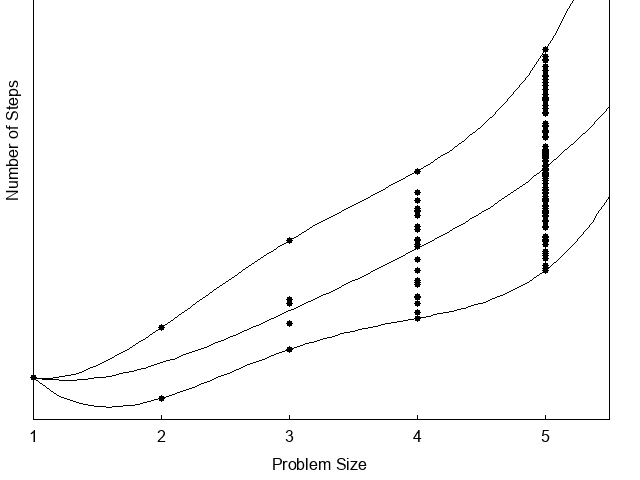
\includegraphics[width=0.75\textwidth]{./assets/imgs/bigOcomplexity.png}
		\caption{\label{fig:bigOgraph} Best, worst and average-case complexity}
	\end{figure}
	
	The worst-case complexity turns out to be the most useful of these measures in practice. At first glance this might seem counter-intuitive Perhaps the best analogy is think about what happens if you bring £$n$ into a casino to gamble. The best case is that you walk out owning the place, it is possible but is so unlikely that you should not even think about it. The worst case, that you lose all $n$ dollars is easy to calculate and distressingly likley to happen. The average case, that the typical bettor loses \SI{87.32}{\percent} of the money that they bring into the casino, is difficult to establish and its meaning is subject to debate. What exactly does \textit{average} mean? Stupid people loose more that smart people, so are you smarter or stupider than the average person, and by how much? Card counters at blackjack do better on average than customers that accept three or more free drinks. It is far easier to avoid all of these complexities and obtain a very useful result just by considering the worst case.
	
	The last important thing to realise is that each of these time complexities define a numerical function, representing time versus problem size. These functions are as well defined as any other numerical function, be it $y = x^2 - 2x + 1$ or the price of a particular stock as a function of time. However time complexities are such complex functions that we must simplify them to work with.  For this we need \enquote{Big Oh} notation. 
\section{Big Oh Notation}
\index{Big Oh Notation}
  The issue with using numerical functions when doing complexity analysis tends to be two fold:
  \begin{itemize}
  	\item \textit{They have two many bumps} - An algorithm such as binary search typically runs a bit faster for arrays of size $n = 2^k - 1$ (where $k$ is an integer), because the array partitions works out nicely. Whilst this detail is not particularly significant, it does mean that the \textit{exact} complexity function is likely to be very complicated, with little up and down bumps. 
  	\item \textit{Requires too much detail to specify precisely} - Counting the exact number of RAM instructions executed in the worst case requires that the algorithm be specified to the detail of a complete computer program. This means that individual foibles of the programming language start to creep in, e.g. the peformance of a \texttt{case} statement in C vs a nested if in Python would start to play a role.  
  \end{itemize}

	\subsection{Formal Definition}
		\begin{figure}[t]
			\centering
			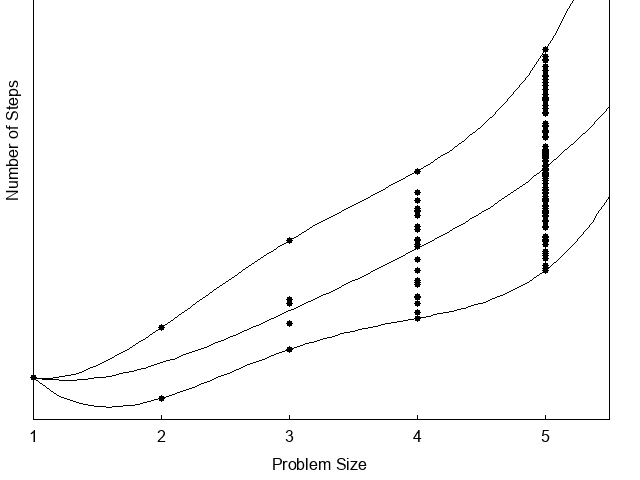
\includegraphics[width=0.75\textwidth]{./assets/imgs/bigOcomplexity.png}
			\caption{\label{fig:bigOdefiniton} Illustrating the Big Oh notations}
		\end{figure}
		The formal definition of Big Oh states that	$f(n) = \mathcal{O}(g(n))$ means $c \cdot g(n)$ is an \textit{upper bound} on $f(n)$. Thus there exists some constant $c$ such that $f(n)$ is always $\le c \cdot g(n)$, for a large enough $n$ (i.e., $n \ge n_0$ for some constant $n_0$). \footnote{We should also add for completeness there is also a function $\Omega(g(n))$ which provides a lower bound, and $\Theta(g(n))$ that exists bounded between $\Omega(g(n))$ and Big Oh.}
		
		But what does that actually mean? First it assumes a constant $n_0$ beyond which they are always satisfied. This means we are not concerned about small values of $n$. This seems reasonable on two fronts: first, most programs take about the same time for $n\le10$ so we are not to concerned with performance; second, there more significant fluctuations that exist for low $n$. We are more concerned how our algorithm behaves at $n=\num{10000}$ and $n=\num{100000}$. Second it is not concerned with any multiplicative constants. The function $f(n) = 2n$ and $g(n) = n$ are identical in big Oh analysis for different values of $c$. Figure \ref{fig:bigOdefiniton} shows how we can draw an upper and lower bound on some function $f(n)$. 
		
		\begin{figure}[t]
			\centering
			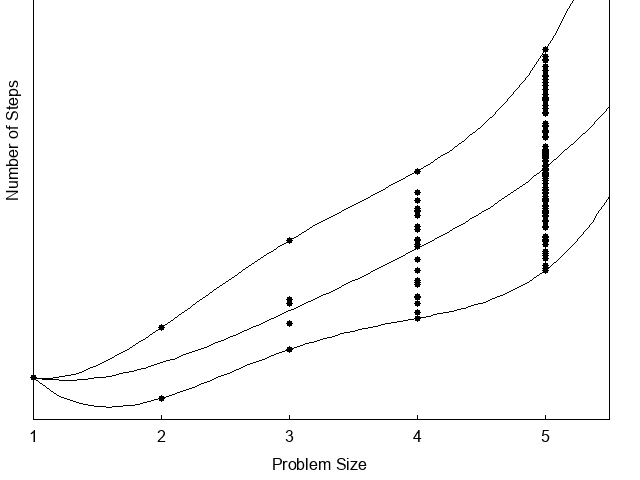
\includegraphics[width=0.75\textwidth]{./assets/imgs/bigOcomplexity.png}
			\caption{\label{fig:bigOExampleGraph} Fitting a function to f(n) for a variety of constants}
		\end{figure}
	
		As an example lets take the function $3n^2 - 100n + 6$, which we've plotted in \ref{fig:bigOExampleGraph}, and try and work out what its big Oh notation is.
		
		\begin{equation}
			3n^2 - 100 + 6 = \bigo{n^2}, \text{for}\: c = 3 \because 3n^2 > 3n^2 - 100n + 6 
		\end{equation}
		\begin{equation}	
			3n^2 - 100 + 6 = \bigo{n^3}, \text{for}\: c = 1 \because n^3 > 3n^2 - 100n + 6\: \text{when}\: n > 3 
		\end{equation}
		\begin{equation}	
			3n^2 - 100 + 6 \ne \bigo{n}, \forall c \because c \cdot n < 3n^2, \text{when}\: n>c
		\end{equation}
		
		The slightly confusing part is when you see the expression $n^2 = \bigo{n^3}$, but if you go back to the definitions and remember that Big Oh is defined in terms of an \textit{upper bound}. This means that we can read the \enquote{=} here as meaning \textit{one of the functions that are}. Clearly $n^2$ is one of the functions that are \bigO{n^3}.
	 
	\subsection{Grow Rates and Dominance Relations}
		With the Big Oh notation, we discard the multiplicative constants, thus the functions $f(n) = 0.001n^2$ and $g(n) = 1000n^2$ are treated identically, even though $g(n)$ is a million times larger than $f(n)$ for all values of $n$. The reason why we are content with the fairly coarse analysis provided in Table \ref{tab:BigOComparison}, which shows the growth rate of several common time analysis functions. In particular it shows how long algorithms that use $f(n)$ operations take to run on a computer that executes one instruction in \SI{1}{\ns} (e.g. \SI{1}{\giga\hertz}). We can draw the following conclusions:
		
		\begin{itemize}
			\item All such algorithms take roughly the same time for $n = 10$
			\item Any algorithm with $n!$ running time becomes useless for $n\ge 20$.
			\item Algorithm whose running time is $2^n$ have a greater operating range, but become impractical for $n>40$.
			\item Quadratic-time algorithms remain usable up to about $n = \num{10000}$, but quickly deteriorate with larger inputs.
			\item Linear-time and $n \lg n$ algorithms remain practical on inputs of one billion item.
			\item A \bigO{\lg n} algorithm hardly breaks a sweat for any imaginable value of $n$.
		\end{itemize}
	
	The bottom line is that despite ignoring constant factors, we get an excellent idea of whether a given algorithm is appropriate for a problem of a given size. 
	
		\subsubsection{Dominance Relations}
			We can group Big notation into a set of classes, such that all the functions in a particular class are equivalent in respect to Big Oh. We say that a faster growing function \textit{dominates} a slower-growing one. Below we shall list the most common function classes in order of increasing dominance.
			%TODO: Expand this Section
			\begin{description}
				\item[Constant functions, $f(n) = 1$] Such functions might measure the cost of adding two numbers, printing out the lyrics to a song, or inserting into a sorted array. There is no dependence on the size of $n$.
				\item[Logarithmic functions, $f(n) = \log n$] This turns up in algorithms such as binary search. They grow quite slowly as $n$ gets big but faster than the constant function.
				\item[Linear functions, $f(n) = n$] Such functions measure the cost of looking at each item once (or twice, or ten times) in an $n$-element array, say to compute the average value.
				\item[Superlinear functions, $f(n) = n \log n$] This class of functions arises in algorithms such as Quicksort and Mergesort.
				\item[Quadratic functions, $f(n) = n^2$] These measure the cost of looking at most or all \textit{pairs} of items in an $n$-element universe. This arises in algorithms such as insertion and selection sort.
				\item[Cubic functions, $f(n) = n^3$] These functions enumerate over all triples of items in an $n$-element universe. 
				\item[Exponential functions, $f(n) = c^n \forall c > 1$] Functions like $2^n$ arise when enumerating all subsets of n items.
				\item[Factiorial functions, $f(n) = n!$] Functions like this arise when generating all permutations or orderings of $n$ items.
			\end{description}
			\begin{figure}[t]
				\centering
				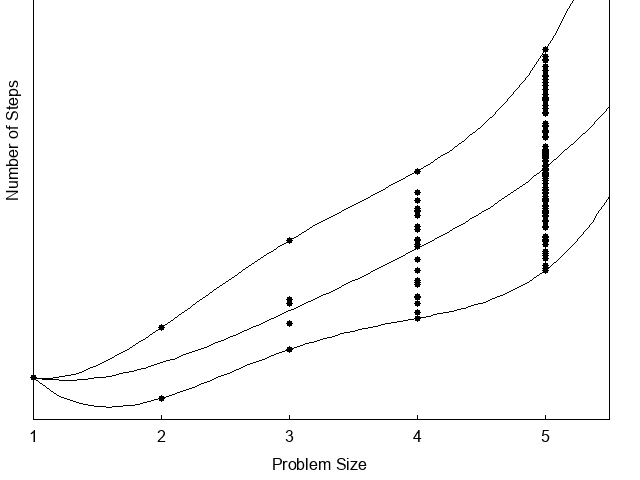
\includegraphics[width=0.8\textwidth]{./assets/imgs/bigOcomplexity.png}
				\caption{\label{fig:bigODominanceRelationships} The growth rates of various common functions}
			\end{figure}			
			Figure \ref{fig:bigODominanceRelationships} shows these graphically. We'll discuss the importance of dominance relationships in the next section. However the important thing to understand is:
			\begin{equation}
				n! \gg c^n \gg n^3 \gg n^2 \gg n \log n \gg n \gg \log n \gg 1
			\end{equation}
		As a shorthand we often refer to problems that have polynomial or less solutions are known as traceable problems and ones with greater than polynomial solutions are called in-traceable.
\begin{table}[t]
	\centering
	\begin{tabular}{>{\scriptsize}L{0.15\linewidth} | >{\scriptsize}L{0.10\linewidth} >{\scriptsize}L{0.10\linewidth} >{\scriptsize}L{0.10\linewidth} >{\scriptsize}L{0.10\linewidth} >{\scriptsize}L{0.10\linewidth} >{\scriptsize}L{0.10\linewidth}}
		\renewcommand{\arraystretch}{0.1}
		$n$				& $\lg n$	& $n$		& $n \lg n$	& $n^2$		& $2^n$		& $n!$		\\
		\hline \hline
		$\num{10}$ 			& \SI{0.003}{\us}	& \SI{0.01}{\us}	& \SI{0.033}{\us}	& \SI{0.1}{\us}		& \SI{1}{\us}		& \SI{3.63}{\ms} 		\\
		$\num{20}$			& \SI{0.004}{\us}	& \SI{0.02}{\us}	& \SI{0.086}{\us}	& \SI{0.4}{\us}		& \SI{1}{\ms}		& \SI{77.1}{\year}		\\
		$\num{30}$			& \SI{0.005}{\us}	& \SI{0.03}{\us}	& \SI{0.147}{\us}	& \SI{0.9}{\us}		& \SI{1}{\s}		& \SI{8.4e15}{\year}	\\
		$\num{40}$			& \SI{0.005}{\us}	& \SI{0.04}{\us}	& \SI{0.213}{\us}	& \SI{1.6}{\us}		& \SI{18.3}{\min}	&						\\
		$\num{50}$			& \SI{0.006}{\us}	& \SI{0.05}{\us}	& \SI{0.282}{\us}	& \SI{2.5}{\us}		& \SI{13}{\day}		&						\\
		\hline
		$\num{100}$			& \SI{0.007}{\us}	& \SI{0.1}{\us}		& \SI{0.644}{\us}	& \SI{10}{\us}		& \SI{4e13}{\year}	&						\\
		$\num{1000}$		& \SI{0.010}{\us}	& \SI{1}{\us}		& \SI{9.966}{\us}	& \SI{1}{\ms}		&					&						\\
		$\num{10000}$		& \SI{0.013}{\us}	& \SI{10}{\us}		& \SI{130}{\us}		& \SI{100}{\ms}		&					&						\\
		$\num{100000}$		& \SI{0.017}{\us}	& \SI{0.10}{\ms}	& \SI{1.67}{\ms}	& \SI{10}{\s}		&					&						\\
		$\num{1000000}$		& \SI{0.020}{\us}	& \SI{1}{\ms}		& \SI{19.93}{\ms}	& \SI{16.7}{\minute}&					&						\\
		$\num{10000000}$	& \SI{0.023}{\us}	& \SI{0.01}{\s}		& \SI{0.23}{\s}		& \SI{1.16}{\day}	&					&						\\
		$\num{100000000}$	& \SI{0.027}{\us}	& \SI{0.1}{\s}		& \SI{2.66}{\s}		& \SI{115.7}{\day}	&					&						\\
		$\num{1000000000}$	& \SI{0.030}{\us}	& \SI{1}{\s}		& \SI{29.90}{\s}	& \SI{31.7}{\year}	&					&						\\
	\end{tabular}
	\caption{\label{tab:BigOComparison} A Comparison of the worst case performances of different implementations of a Dictionary for different operations.}
\end{table}
	\subsection{Working with the Big Oh}
		When reasoning what Big Oh class different 	
		\subsubsection{Adding Functions}
			The sum of two functions is governed by the dominant one, i.e
			\begin{equation}\label{equ:bigOaddingdominance}
				\bigo{f(n)} + \bigo{g(n)} \rightarrow \bigo{\max(f(n),g(n))}
			\end{equation}
		
		\subsubsection{Multiplying Functions}
			There are two types of multiplication that we need to worry about with Big Oh, the first is with a constant factor, the second is with a second function. With a constant the answer is simple, you just ignore it as in Equation \ref{equ:bigOmultiplicationconstant}. Obviously this doesn't hold for $c \ge 0$ as multiplying even \bigO{n!!} is quickly wiped out if you multiply it by zero, but for most cases we will come across this will not be the case.
			
			\begin{equation}\label{equ:bigOmultiplicationconstant}
				\bigo{c \cdot f(n)} \rightarrow \bigo{f(n)}
			\end{equation}
			
			However for when you are multiplying a function by another function both results are important. This leads to the result in Equation \ref{equ:bigOmultiplicationfunction}. 
			
			\begin{equation}\label{equ:bigOmultiplicationfunction}
				\bigo{f(n)} \cdot \bigo{g(n)} \rightarrow \bigo{f(n) \cdot g(n)}
			\end{equation}
			e.g.
			\begin{equation}\label{equ:bigOmultiplicationfunctionexample}
			\bigo{n^2} \cdot \bigo{\log n} \rightarrow \bigo{n^2 \log n}
			\end{equation}
			
		

			
	\subsection{Example Derivation}
		In this section we are going to reason our way through some common algorithms and see if we can derive the big Oh notation for a given algorithm.
		\subsubsection{String Pattern Matching}
			Pattern matching is the most fundamental algorithm that we perform on text strings. This algorithm implements the find command available in any web browser or text editor.
			
			\textit{Problem:} Substring Pattern Matching
			\textit{Input:} A text string $t$ and a pattern string $p$.
			\textit{Output:} Does $t$ contain the pattern $p$, and if so where?
			
			\begin{figure}[h]
\begin{minted}{c}
int findmatch(char *p, char *t) {
	int i, j;		/* counters */
	int m, n;		/* string lengths */
	
	m = strlen(p);
	n = strlen(t);
	
	for (i=0; i <= (n - m); i++) {
		j = 0;
		while((j < m) && (t[i+j] == p[j])) {
			j = j+1;
		}
		if (j == m) {
			return(i);			
		}
	}
	
	return(-1);
}
\end{minted}
				\caption{\label{code:findmatch} Algorithm for finding a matching string.}
				\index{Strings!Substring}
			\end{figure}
				
			What is the worst-case running time of these two nested loops? The inner \textit{while} looop goes around at most $m$ times, and potentially far less when the pattern match fails. The outer loop goes around at most $n-m$ times, since no complete match can be found once there are not enough characters left. With nested loops we multiply the complexity \footnote{This is because every time we run the outer the loop we run the complete inner loop} so we get a worst case complexity given in equation \ref{equ:findmatch1}, the $+2$ refers to the two extra statements that are within the outer \textit{for} loop.
			
			\begin{equation}\label{equ:findmatch1}
				\bigo{(n-m)(m + 2)}
			\end{equation}
			
			We also need to consider the time taken to find the length of each of the strings. Lets just assume that we explicitly count the number of characters until we hit the end of the string, this suggests that it would take linear time. So the total running time would be given in equation \ref{equ:findmatch2}
			\begin{equation}\label{equ:findmatch2}
			\bigo{n+m+(n-m)(m + 2)}
			\end{equation}
			
			Simplifying the constant term,
			\begin{equation}\label{equ:findmatch3}
			\bigo{n+m+(n-m)m}
			\end{equation}
			
			Multiplying it out,
			\begin{equation}\label{equ:findmatch4}
			\bigo{n+m+nm-m^2}
			\end{equation}
			
			We know that $n \ge m$ because a sub string that longer than the original text would be impossible. So,
			\begin{equation}\label{equ:findmatch5}
			n + m \le 2n \rightarrow \bigo{n}
			\end{equation}
			Substituting \ref{equ:findmatch5} in leaves:
			\begin{equation}\label{equ:findmatch6}
			\bigo{n+nm-m^2}
			\end{equation}
			We also note that $n \le nm$, since $m \ge 1$ for any interesting problem thus:
			\begin{equation}\label{equ:findmatch7}
			n + nm \rightarrow \bigo{nm}
			\end{equation}
			This allows us to drop the additive $n$ and leave us with Equation \ref{equ:findmatch8}
			\begin{equation}\label{equ:findmatch8}
			\bigo{nm-m^2}
			\end{equation}
			Finally we observe that the $-m^2$ term is negative so only serves to lower the value within. Because Big Oh is an upper bound, we can drop any negative without invaliding the output. We also know that because $n \ge m$, $ mn \ge m^2$ so it isn't big enough to cancel out any term that is left. This leaves a worst case complexity of \bigO{nm}
			
		\subsubsection{Matrix Multiplication}
			Matrix multiplication is a fundamental operation in linear algebra. 
			\textit{Problem:} Matrix Multiplication
			\textit{Input: } Two matrices, $A$ (dimensions $x \times y$) and $B$ (dimensions $y \times z$)
			\textit{Output: } A $x \times z$ matrix $C$ where $C[i][j]$ is the dot product of the $i$th row of $A$ and the $j$th column of $B$.
			
			\begin{figure}[h]
\begin{minted}{c}
for (i = 1; i <= x; i++) {
	for (j = 1; j <= z; j++) {
		C[i][j] = 0;
		for (k = 1; k <= y; k++) {
			C[i][j] += A[i][k] * B[k][j];		
		}
	}
}
\end{minted}
				\caption{\label{code:matrixmult} Multiplying two matrices, A and B to get C.}
			\end{figure}
		
			The number of multiplication operations is given by $M(x, y, z)$ which is the result of a nested summation shown in \ref{equ:matrixmult1}
			
			\begin{equation}\label{equ:matrixmult1}
				M(x,y,z) = \sum_{i=1}^{x} \sum_{j=1}^{y} \sum_{k=1}^{z} 1 	
 			\end{equation}
 			We evaluate from the right inward. The sum of $z$ ones is $z$ so:
 			\begin{equation}\label{equ:matrixmult2}
	 			M(x,y,z) = \sum_{i=1}^{x} \sum_{j=1}^{y} z
	 		\end{equation}
	 		\begin{equation}\label{equ:matrixmult3}
	 			M(x,y,z) = \sum_{i=1}^{x}yz
	 		\end{equation}
		 	\begin{equation}\label{equ:matrixmult4}
	 			M(x,y,z) = xyz
 			\end{equation}
	 		
	 		Thus the running of a matrix multiplication \index{Matrix Multiplication} is \bigO{xyz}, for the case that $x = y = z$ we get \bigO{n^3} i.e. a cubic algorithm.
		\subsubsection{Binary Search and Logarithms}
			Binary Search \index{Binary Search} is a good example of an \bigO{\log n} algorithm. It is covered in more detail in section \ref{section:BinarySearch} but for now imagine you have a telephone book. You want to locate person, $p$ in a telephone book containing $n$ names. In a binary search you start by comparing it to the middle or \nicefrac{n}{2} name, say \textit{Monroe, Marilyn}. You then discard half the book depending if the name came before or after middle. You repeat this process until you get to having only one name left. The important question for our analysis is how many steps will it take to get down to this one name? 
			Lets start by turning the problem on its head. After $h$ comparisons how many different values could you have compared? For $h = 1$ the answer is trivial - 1. For $h = 2$, we have the first element that we compared and the two either that we jump to next. Fig \ref{fig:simpleBinaryTree} demonstrates how the number of items grows for $h$. We can work out that after $h$ jumps we can cover $2^h - 1$ items. Equation \ref{equ:binSearch1} shows how this is derived to get a complexity of \bigO{\lg n}
			\begin{gather}
				n = 2^h - 1 \label{equ:binSearch1} \\
				\lg n = \lg(2^h) - \lg 1 \label{equ:binSearch2} \\
				\lg n = h \label{equ:binSearch3}
			\end{gather}
			
			\begin{figure}[t]
				\centering
				\begin{tikzpicture}
					\draw[fill=black] (0,0) circle (0.05)  node[above] {\small Monroe, Marlyin};
					\draw[fill=black] (-3,-1) circle (0.05)  node[above] {\small Dean, James};
					\draw[fill=black] (3,-1) circle (0.05)  node[above] {\small Presly, Elvis};
					\draw[fill=black] (-4.5,-2) circle (0.05)  node[above] {\small Collins, Phil};
					\draw[fill=black] (-1.5,-2) circle (0.05)  node[above] {\small Hendrix, Jimmi};
					\draw[fill=black] (1.5,-2) circle (0.05)  node[above] {\small Parton, Dolly};
					\draw[fill=black] (4.5,-2) circle (0.05)  node[above] {\small Springsteen, Bruce};
					
					\draw[->] (-7,1)  node[above]  {$h$} -- +(0,-5);
					\draw (-7,0) -- +(-.2,0) node[left] {$1$};
					\draw (-7,-1) -- +(-.2,0) node[left] {$2$};
					\draw (-7,-2) -- +(-.2,0) node[left] {$3$};
					\draw (-7,-3) -- +(-.2,0) node[left] {$\dots$};
					\draw(0,0) -- (-1.75,-0.4);
					\draw(0,0) -- (1.75,-0.4);
					\draw(-3,-1) -- (-3.8,-1.4);
					\draw(3,-1) -- (3.8,-1.4);
					\draw(-3,-1) -- (-2.2,-1.4);
					\draw(3,-1) -- (2.2,-1.4);
				\end{tikzpicture}
				\caption{\label{fig:simpleBinaryTree} the results of a possible Binary Search after $h$ comparisons. }
			\end{figure}
	\section{Greedy Algorithms}
	
	\section{P vs NP Problems}
		One of the most profound open problems in computer science asks \enquote{Is $P = NP$?}. In simple language it is asking whether \textit{verification} is easier than initial \textit{discovery}. A good analogy is lets say during the course of an exam you happen to notice the answer of the student next to you. Are you now better off? You wouldn't turn it in without checking, since you could answer the question correctly if you took enough time to find it from scratch. The question is whether you can really verify the answer faster than you could find it from scratch. 
		
		In particular we are referring to two classes of problems: $P$ and $NP$. The class $P$ is an exclusive club that can only be joined whence a problem has demonstrated that there is a polynomial-time algorithm to solve it. A less-exclusive club welcomes all problems who can be \textit{verified} in polynomial time. This obviously includes all members P. We call this club $NP$ standing for \textit{non-deterministic polynomial time}. The question is whether problems in $NP$ that cannot be in $P$. Most people who actually study this field believe that $P \ne NP$ but haven't found a proof yet.
	
	\section{The Halting Problem}
		So far all the problems that we have covered
	\section{Turing Machines}
	
	\section{State Transition Diagrams}
	
	\section{Exercises}
		
		\subsection{Exam Style Questions}
			\begin{enumerate}
				\item What value is returned by the following function? Express your answer as a function of $n$. Give the worst-case running time using the Big Oh notation
			\end{enumerate}
	% !TeX root = ../main.tex

\chapter{Data Structures}
Data structures


We can class Data structures into two distinct category's based on whether or not they use pointers:
\begin{itemize}
	\item \textit{Contiguously-allocated structures} are composed of single slabs of memory, and include arrays, matrices, heaps and hash tables
	\item \textit{Linked data structures} are composed of distinct chunks of memory bound together by \textit{pointers} and include lists, trees and graph adjacency lists.
\end{itemize}

\section{Arrays}
	The \textit{array} is the fundamental contiguously-allocated data structure. Arrays are structures of fixed-size data records such that each element can be efficiently located by its \textit{index}.

	There are several advantages to using contiguously-allocated arrays:
	\begin{description}
		\item[Constant-time access given the index] - Because the index of each element maps directly to a particular memory address, we can access arbitray data tiems instantly provided we know the index.
		\item[Space Effciency] - Arrays consist purely of data, sono space is wasted with links or other formatting information. Further, end-of-record information is not needed because arrays are built from fixed-size records
		\item[Memory locality] - A common programming idiom involves iterating through all the elements of a data structure. Arrays are good for this because they exhibit excellent memory locality. Physical continuity between successive \textit{cache memory} in modern computer architectures
	\end{description}

	The disadvantages of arrays is that we cannot adjust their size in the middle of a programs' execution. Our program will fail soon as we try to add the $(n+1)$ customer, if we have only allocated room for $n$ records. We could compensate by allocating extremely large arrays, but this can waste space, restricting what our programs actually do.

	\subsection{Dynamic Arrays}
		Dynamic Arrays are a way around the restriction placed by arrays being fixed size. With a dynamic array we enlarge arrays as we need them. Suppose we start with an array of size 1, and double its size from $m$ to $2m$ each time we run out of space. This doubling process involves allocating a new array of size $2m$, copying the contents of the old array to the lower half of the new one, and returning the space used by the old array to the storage allocation system. Snippet. \ref{code:doubleArray} shows an implementation that takes an array and a size and returns a new array.
\begin{listing}[h]
	\begin{minted}{c}
int* double_array(int *array, int size) {
	int i;
	int* new_array = malloc(sizeof(int) * 2 * size);
	for(i = 0; i < size; i++) {
		new_array[i] = array[i]
	}
	free(array);
	return new_array;
}
	\end{minted}
	\caption{\label{code:doubleArray} Implementing a dynamic array in C}
\end{listing}

	On average each of the $n$ elements in the array only move $2n$ times, so the total work is the on the order of \bigO{n}. Adding a new element to an array no longer takes constant time \textit{in the worst case} instead all querys will be fast, except for those relatively few queries triggering array doubling.

\section{Linked Lists}
	Linked lists are one of the fundemental data structures which are often extended to make complex structures.
\begin{listing}[h]
	\begin{minted}{c}
typedef struct list {
	item_type  item; // data item
 	struct list *next; // pointer to successor
}
\end{minted}
	\caption{\label{code:linkedlist} Linked List declaration}
\end{listing}
	All linked data structures share certain properties as shown in snippet \ref{code:linkedlist}. In particular:
	\begin{itemize}
		\item Each node in our data structure (here \texttt{list}) contains one or more data fields (here \texttt{item}) that retain the data that we need to store
		\item Each node contains a pointer field to at least one other node (here \texttt{next}). This means that much of the space used in linked data structures has to be devoted to pointers, not data.
		\item Finally, we need a pointer to the head of the structure so that we know where to start.
	\end{itemize}

	The list is the simplest linked structure. The three basic operations supported by lists are searching, insertion and deletion. In doubly-linked lists, each node points to both its successor and its predecessor

	\begin{figure}[h]
		\centering
		\begin{tikzpicture}
		\draw [fill=gray!80]  (-5,0.5) node (v4) {}  ellipse (0.5 and 0.5);
		\draw  (-3,1) rectangle (-1,0) node (v1) {};
		\draw  (v1) rectangle (0,1);
		\draw  (1.5,1) rectangle (3.5,0) node (v2) {};
		\draw  (v2) rectangle (4.5,1);
		\draw  (6,1) rectangle (8,0) node (v3) {};
		\draw  (v3) rectangle (9,1);
		\draw[-stealth, thick] (-0.5,0.5) -> (1.5,0.5);
		\draw[-stealth, thick]  (4,0.5) -- (6,0.5);
		\draw[-stealth, thick]  (v4) -- (-3,0.5);
		\node at (-2,0.5) {Brown};
		\node at (2.5,0.5) {Cameron};
		\node at (7,0.5) {May};
		\node at (8.5,0.5) {NIL};
		\end{tikzpicture}
		\caption{\label{fig:singlylinkedlist} a singly linked list for the 3 most recent prime minsters}
	\end{figure}

	\subsection{Searching a List}
		Searching for item $x$ in a linked list can be done either utilising iteration or recursion. Snippet. \ref{code:search_list} is an example of a recursive implementation. If $x$ is in the list it is either in the first item or it is located in the smaller rest of the list. Eventually we will reach a point where we have an empty list. Clearly $x$ cannot be there so we can return $NULL$.
	\begin{listing}[h!]
		\begin{minted}{c}
list* search_list(list *l, item_type x) {
	if (l == NULL) {
		return(NULL);
	}

	if (l->item == x) {
		return(l);
	} else {
		return( search_list(l->next, x));
	}
}
\end{minted}
	\caption{\label{code:search_list} Searching for item $x$ in list $l$}
\end{listing}

		\subsection{Insertion into a list}
			Insertion into a list is. We have no particular need at this moment to maintain the list in any particular order so we can instead choose to insert each new item where ever is easiest. In a singly linked list this is the beginning as it avoids any need to traverse the list, but does require us to update the pointer at the end of the list, denoted $l$. Snippet. \ref{code:insert_list} shows the pointer manipulation required. Just a quick note, the double star ($\texttt{**l}$) denotes that $l$ is a \textit{pointer to a pointer} to a list node. Thus the last line, \texttt{*l=p;}, copies $p$ to the place pointed to by $l$, which is the external variable maintaining access to the head of the list.

\begin{listing}[h!]
	\begin{minted}{c}
void insert_list(list **l, item_type x) {
	list *p; /* temporary pointer */
	p = malloc( sizeof(list));
	p-> item = x;
	p-> next = *l;
	*l = p;
}
\end{minted}
	\caption{\label{code:insert_list} Inserting item $x$ into list $l$}
\end{listing}

	\subsection{Deletion from a List}
		Deletion from a linked list is a bit more complicated than insertion. First we don't have the luxury of just deleting where ever is easiest. Instead we have to search to find the pointer to the \textit{predeccessor} of the item to be deleted. Snippet. \ref{code:predecessor_list} shows how we can use recursion to find the necessary pointer.

\begin{listing}[h!]
	\begin{minted}{c}
list predecessor_list(list *l, item_type x) {
	if((l == NULL) || (l->next == NULL)) {
		retur(NULL);
	}

	if ((l->next)->item == x) {
		return(l);
	} else {
		return( predecessor_list(l->next, x));
	}
}
\end{minted}
	\caption{\label{code:predecessor_list} Finding the predecessor to item $x$ in list $l$}
\end{listing}

Now that we have found the pointer to the doomed node, the actual deletion operation is simple, once ruling out the case that the to-be-deleted element doesn't exist. Note that special care should be taken to reset the pointer to the head of the list ($l$) when the first element is deleted.

\begin{listing}[h!]
	\begin{minted}{c}
void delete_list(list **l, item_type x) {
	list *p;			/* item pointer */
	list *pred; 		/* predecessor pointer */
	list *search_list(), *predecessor_list();

	p= search_list(*l, x);
	if (p != NULL) {
		pred = predecessor_list(*l, x);
		if (pred == NULL) {
			*l = p->next; /* Case when x is head */
		} else {
			pred->next = p->next;
		}
		free(p);
	}
}
\end{minted}
	\caption{\label{code:delete_list} Deleting item $x$ from list $l$}
\end{listing}

\section{Comparison of Arrays and Linked Lists}
	The relative advantages of linked lists over static arrays include:
		\begin{itemize}
			\item Overflow on linked structures can never occur unless memory is actually full.
			\item Insertions and deletions are simpler than for contiguous (array) lists.
			\item With large records, moving pointers is easier and faster than moving the items themselves
		\end{itemize}
	The relative advantages of arrays include:
	\begin{itemize}
		\item Linked structures require extra space for storing pointer fields.
		\item Linked lists do not allow efficient random access to items
		\item Arrays allow better memory locality and cache performance than random pointer jumping.
	\end{itemize}

\section{Fields, Records and Files}
	
	\subsection{Fields and Records}
	
	\subsection{Text Files}
		\subsubsection{CSV}
		
		\subsubsection{XML}
		
		\subsubsection{JSON}
		
	\section{Binary Files}
\section{Abstract Data Types}
\section{Stacks and Queues}
	Stacks and Queues are often called \textit{containers}, denoting that they are data structure that permits storage and retrieval of data items \textit{independent of content}. We distinguish between containers by the particular retrieval order that they support.
	\begin{description}
		\item[Stacks] Support retrieval by last-in, first-out (LIFO) order. Stacks are simple to implement and very efficient For this reason stacks are probably the best container to use when retrieval order doesn't matter. The \textit{put} and \textit{get} operations are often called \textit{push} and \textit{pop}.
		\item[Queues] Support retrieval by first in, first out (FIFO) order. This is usually the fairest way to control waiting times for services. You want the container holding jobs ina FIFO order to minimize the \textit{maximum} time spent waiting. Queues are somewhat trickier to implement than stacks and thus are more appropriate for applications where the order is important. The \textit{put} and \textit{get} operations are often called \textit{enqueue} and \textit{dequeue}.
	\end{description}

	Stacks and queues can be effectively implemented using either arrays or linked lists. The key issue is whether an upper bound on the size of the container is known in advance.

\section{Dictionaries}
	The \textit{dictionary} data type permits access to data items by content. You stick an item into a dictionary so you can find it where you need it. The primary operations of dictionary support are:
	\begin{itemize}
		\item \textit{Search(D,k)} - Given a search key, $k$, return a pointer to the element in dictionary $D$ whose key value is $k$, if one exists.
		\item \textit{Insert(D,x)} - Given a data item $x$, add it to the set in the dictionary $D$.
		\item \textit{Delete(D,k)} - Given a pointer to a given data item $x$ in the dictionary $D$, remove it from $D$.
	\end{itemize}

	Certain dictionary data structues also efficently support other useful operations:
		\begin{itemize}
			\item \textit{Max(D) or Min(D)} - Retrieve the item with the largest (or smallest) key from $D$. This enables the dictionary to serve as a priority queue.
			\item \textit{Predecessor(D,x) or Successor(D,x)} - Retrieve the item from D whose key is immediately before (or after) $x$ in sorted order. This allows us to iterate through the elements of the data structure.
		\end{itemize}
	\subsection{Using a List or an Array?}

		In this section we will look at the advantages and disadvantages or using arrays or linked list for implementing a Dictionary. There are more complicated approaches using binary search trees and hash tables which we will come across shortly. Table \ref{tab:BigODictionary} shows a comparison of the worst case performance of the basic dictionary operations. We will discuss the results of this and the implementations of each of the operations to fully grasp it.
		\begin{table}[h]
				\centering
				\renewcommand{\arraystretch}{1.5}
			\begin{tabular}{M{0.25\linewidth} | M{0.12\linewidth} |M{0.12\linewidth} |M{0.12\linewidth} |M{0.12\linewidth} |M{0.12\linewidth}|M{0.12\linewidth}}
				Dictionary Operations & Unsorted Array & Sorted Array & Singly Unsorted List & Doubly Unsorted List & Singly Sorted List & Double Sorted List \\
				\hline \hline
	$Search(L, k)$ 		& \bigO{n} 	& \bigO{\log n}	& \bigO{n}	& \bigO{n} 	& \bigO{n} 	& \bigO{n} \\
	$Insert(L, x)$ 		& \bigO{1} 	& \bigO{n} 		& \bigO{1} 	& \bigO{1} 	& \bigO{n} 	& \bigO{n} \\
	$Delete(L, x)$ 		& \bigO{1}* & \bigO{n} 		& \bigO{n}* & \bigO{1} 	& \bigO{n}*	& \bigO{1} \\
	$Successor(L, x)$ 	& \bigO{n} 	& \bigO{1} 		& \bigO{n} 	& \bigO{n} 	& \bigO{1} 	& \bigO{1} \\
	$Predecessor(L, x)$	& \bigO{n} 	& \bigO{1} 		& \bigO{n} 	& \bigO{n} 	& \bigO{n}*	& \bigO{1} \\
	$Max(L)$ 			& \bigO{n} 	& \bigO{1} 		& \bigO{n} 	& \bigO{n} 	& \bigO{1} 	& \bigO{1} \\
	$Min(L)$ 			& \bigO{n} 	& \bigO{1} 		& \bigO{n} 	& \bigO{n} 	& \bigO{1}* & \bigO{1} \\
			\end{tabular}
			\caption{\label{tab:BigODictionary} A Comparison of the worst case performances of different implementations of a Dictionary for different operations.}
		\end{table}
	\begin{description}
		\item[Search] For an unsorted array A search is implemented by testing $k$ against (potentially) each element in the array [Linear Search]. In an sorted array you can then use a Binary search giving a worst case performance of $\log n$. In a liked list sorting doesn't  provide the same benefits. Binary Search is no Longer possible, because we can't access the middle element without traversing all the elements before it. However with a sorted list we can quickly terminate the search for items that are not in the array. For example if you were searching for $Major, John$ and reached $May, Theresa$ we can deduce that he doesn't exist in the dictionary. However in the worst case, say searching for $Zebra$ it still must take linear time.
		\item[Insertion] For the unsorted array, insertion is an easy process, you need to increment the size of the array $n$ and then add the new item to the bottom of the array. Similarly for unsorted arrays you can just add the item to the end of the dictionary, which takes constant time. For sorted arrays you need to make room for a new item, which may require moving many items causing insertion to become a linear-time operation. For sorted list, adding a new item is a relatively simple process. However you still need to search for the correct place in the dictionary, taking constant time.
		\item[Deletion] We are given an pointer to the element to be deleted, which is a relatively simple process when dealing with an array. However it does leave a whole that needs to be filled. For an unsorted array you can just write over $A[x]$ with $A[n]$, however for the sorted variation you will need to move each of the elements $A[x+1]$ to $A[n]$ up one position taking constant time. For singly sorted lists the pointer $x$, isn't want we need to remove the element. Instead we need to the pointer to the successor, this will take linear time as we will have to search through all the elements to get to its successor. For doubly linked list this is a simpler operation than sorted arrays as removing an item from a list is an easier problem than filling a hole by moving array elements.
		\item[Traversal Operations (Predecessor and Successor)] refer to the item appearing before $x$ in \textbf{sorted order}. Thus for a sorted array the answer is $A[x-1]$ and $A[x+1]$. For sorted arrays this requires more searching as you need to find the item that is bigger or smaller than $x$. We have a similar issue with unsorted lists and sorted lists. However we again have the problem with lacking a pointer to $x-1$ for the singly linked list, requiring a computationally expensive search to get the required item.
		\item[Maximum and Minimum] We face a similar issue with finding the largest/smallest item as we did with finding successors and predecessors. For sorted arrays the answer is simply $A[n]$ and $A[1]$ respectively. For a sorted doubly linked list the answer is the head and foot element. For other implementations at least one of the operations will require a linear sweep to get the required element.
	\end{description}

\section{Binary Trees}
\index{Binary Trees}
	Binary Trees are a type of data structure that allow for both fast search (like sorted arrays) and flexible updates (like linked lists). Binary Search, discussed further in section \ref{section:BinarySearch} (\pageref{section:BinarySearch}) requires that you have fast access to two elements. Specifically the median elements above and below the given node.

	A \textit{rooted binary tree} is recursively defined as either being:
	\begin{itemize}
		\item empty
		\item Consisting of a node called the root, together with two rooted binary trees called left and right sub-trees respectively.
	\end{itemize}
	The order amongst the two daughter nodes matters in rooted trees, so left is different from right.
	In a binary \textit{search} tree each node has a label that is asingle key such that for any node labelled $x$ , all nodes in the left subtree of $x$ have keys $< x$ and all the nodes in the right subtree of $x$ have keys $> x$. This search tree labelling is very speial. For any binary tree on $n$ nodes and any set of $n$ keys, there is exactly one labelling that gives that makes it a binary search tree.

	\subsection{Implementing a Binary Search Tree}
	Each binary tree node has a \textit{left} and \textit{right} pointers, an opitonal \textit{parent} pointer and a data field. We can then define a tree structure as below:

	\begin{listing}[h]
		\begin{minted}{c}
	typedef struct tree {
		item_type		item;
		struct tree *parent;
		struct tree *left;
		struct tree *right;
	} tree;
		\end{minted}
		\caption{\label{code:structtree} Structure of a tree node with optional parent parameter}
	\end{listing}

	The basic operations supported by a binary tree are searching, traversal, insertion, and deletion.
		\subsubsection{Searching in a Tree}
	To find a particular node in a binary search tree you start from the root node and work your way down the tree. For a given key $k$, and a node that has a value of $x$, there are 3 possible outcomes.
	\begin{itemize}
		\item  - Return current node
		\item  - Go to the right subtree
		\item  - Go to the left subtree
	\end{itemize}
	Because each subtree of a binary tree is itself a binary search tree we can move through the tree recursively. Below you'll find a search algorithm that runs in \bigO{h} time, where $h$ denotes the height of the tree.

	\begin{listing}[h]
		\begin{minted}{c}
tree *search_tree(tree *l, item_type x) {
	if (l == NULL) return NULL;

	if (l->item == x) return(l);

	if (x < l->item) {
		return( search_tree(l->left, x) );
	}
	else {
		return( search_tree(l->right, x) );
	}
}
\end{minted}
		\caption{\label{code:structtree} Structure of a tree node with optional parent parameter}
	\end{listing}
	This algorithm runs in \bigO{h} time, where $h$ is the height of the tree.
		\subsubsection{Finding the Minimum and Maximum itemize}
	A special case of searching is finding the maximum and minimum elements in the tree. By definition the smallest element in the tree must be in the left subtree as all keys in the left subtree must have values less than that of the root. Applying this logic recursivly leads to the conclusion that the smallest item must be on the leftmost decendant on the root. Similarly, the maximum item must be on the rightmost descendant
	\begin{listing}[h]
		\begin{minted}{c}
tree *find_minimum(tree *t) {
	tree *min; //pointer to minimum elements

	if (t == NULL) return(NULL);

	min = t;
	while (min -> left != NULL) {
		min = min->left;
	}
	return(min);
}
		\end{minted}
		\caption{\label{code:findmintree} The find minimum function.}
	\end{listing}

\subsubsection{Traversal of a Tree}
		% Visiting all the nodes in a binary search tree turns up in many important algorithms. A prime application of tree traversal is listing the labels of the tree nodes. Binary search trees make it easy to report the labels in sorted order. By definition all the keys smaller than the root must lie in the left subtree of the root and all keys bigger than the root in the right subtree. Thus, visiting all the nodes recursively produces an \textit{in-order} traversal of the search tree. Note that the function \texttt{process_item} 
		\citet{Boole54}
\begin{listing}[h]
	\begin{minted}{c}
void traverse_tree (tree *l) {
	if (l != NULL) {
		traverse_tree(l->left);
		process_item(l->item);
		traverse_tree(l->right);
	}
}
	\end{minted}
	\caption{\label{code:inordertraversal} The traversing a binary tree in order..}
\end{listing}
			\subsubsection{Insertion in a Tree}
			\subsubsection{Deletion from a Tree}
		\subsection{Balanced Binary Search Trees}
\section{Priority Queues}
\section{Hashing and Strings}
	\subsection{Collision Resolution}
		
\section{Graphs}
	\subsection{Flavours of Graphs}
	\subsection{Data Structures for Graphs}
	
		\subsubsection{Adjacency Matrix}
		
		\subsubsection{Adjacency Lists}


\section{Vectors}

	\subsection{Dot Product}
	
	\subsection{Angle Between Vectors}
	
\section{Exercises}
\subsection{Exam Style Questions}

\subsection{Programming Challenges}
%\begin{enumerate}
%	\item A common problem for compilers and text editors is determining whether the parentheses in a string are balanced and properly nested. For example, the string \texttt{((())())()} contains properly nested pairs of parentheses, which the strings \texttt{)()(} and \texttt{())} do not.
%
%	Give an algorithm that returns true if a string contains properly nested and balanced parentheses, and false if otherwise.
%
%	\bonus Identify the position of the first offending parenthesis if the string is not properly nested and balanced.
%	\item What changes would have to be made to Snippet. \ref{code:findmintree} to implement a find_maximum function for a binary search tree?
%\end{enumerate}

	\chapter{Algorithms}

	\section{Searching}
	
		\subsection{Linear Search}
		
		\subsection{\label{section:BinarySearch}Binary Search}
		
			\subsubsection{Binary Tree Search}
			
	\section{Sorting}
		
		\subsection{Bubble Sort}
		
		\subsection{Merge Sort}
		
		\subsection{Insertion Sort}
		
		\subsection{Quick Sort}
		
	\section{Graph Traversal}
	
		\subsection{Breadth First}
		
		\subsection{Depth First}
		
		\subsection{Dijkstra}
		
		\subsection{A Star}
		
		\subsection{Floyd-Warshall}

\part{The Physical Computer}
	\chapter{Hardware}
	\section{Relationship between Hardware and Software}
	
	\section{Main Memory}
	
		\subsection{Stored Program Concept}
			What separates computers from other machines is their ability to perform an infinite array of tasks, from interactive games, to word processing and performaing scientific calculations, all without needing change hardware . A washing machine contains a basic processor to control the different cycles and temperatures, but trying to get it to perform even a basic calculation you will struggle. This flexibility comes down to a concept known as the \index{Stored Program} \textit{Stored Program} concept. The idea behind it is remarkably simple, you have a fixed hardware platform capable of executing a fixed repertoire of instructions. At the same time these instructions can be used and combined to create arbitrary sophisticated programs. Moreover, the logic of these programs are not embedded in hardware, as it was in early computers, instead they are stored and manipulated in the computer's memory.   
		\subsection{Addressable Memory}
		
	\section{Secondary Storage}
		
		\subsection{Hard Disk Drive}
		
		\subsection{Solid State Drive}
			
			\subsubsection{NAND Flash Memory}
			
			\subsubsection{SSD Controller}
			
			\subsubsection{Pages}
			
		\subsection{Optical Drive}
		
	
	\chapter{The Processor}
	\section{The Little Man Computer}
		The power of the computer does not arise from complexity, instead it comes from its ability to perform simple operations at an extremely high rate of knots. This means that actual design of a computer is also simple. We'll start our adventure in investigating the processor by looking at the Little Man Computer (LMC). Whilst it is not a physical computer it is a simplified model to allow us to understand the basics of computer architecture before moving on to looking at the more complex RM processor.
		
			\subsection{Physical Layout}
				\begin{figure}[t]
					\begin{center}
						\begin{tikzpicture}[scale = 0.5]
							\draw[ultra thick] (0,4.5) -- (0,0) -- (20,0) -- (20,15) -- (0,15) -- (0,10.5);
							\draw [ultra thick] (0,9.5) -- (0,5.5);
							\draw [ultra thick] (-0.5,10.5) -- (0.5,10.5);
							\draw [ultra thick] (-1.5, 10.5) -- (-1,9.5) -- (1,9.5) -- (1.5, 10.5);
							
							\draw [ultra thick] (-0.5,5.5) -- (0.5,5.5);
							\draw [ultra thick] (-1.5, 5.5) -- (-1,4.5) -- (1,4.5) -- (1.5, 5.5);
							
						\end{tikzpicture}
					\end{center}
					\caption{\label{fig:LMCLayout} Layout of the Little Man Computer}
				\end{figure}
				We shall start by looking at the physical layout of the Little Man Computer, illustrated in Fig. \ref{fig:LMCLayout}. The LMC consists of a walled post-room, indicated by thick line. Inside this their are various items.
				\begin{itemize}
					\item \num{100} \textit{pigeon holes} - numbered with an address ranging from \numrange[minimum-integer-digits=2]{00}{99}. Each pigeon hole is designed to hold a single slip of paper, upon which is written a three digit decimal number. 
					\item  \textit{A Calculator} - the calculator is used to enter and temporarily hold numbers, and also to add or subtract. The display is three digits wide and there is no provision made for negative numbers
					\item A \textit{Hand Counter} - The type that you click to increment the count. There is a reset button located outside the post-room.
					\item The \textit{Little Man} - It is his role to perform certain tasks to be defined shortly.
					\item An \textit{in basket} and an \textit{out basket}. These allow a user to communicate with the Little Man by putting a three digit number into the in basket. Similarly the out box allows the Little Man to write a three digit number on a slip of paper and leave it in the out basket.
				\end{itemize} 
				
			\subsection{Instructions of the LMC}
				We would like the Little Man to do some useful work for us. For this purpose we have invented a small group of instructions that he can perform. Each instruction will consist of 3 digits. We use the first digit to tell the Little Man what instruction to perform, this is known as the opcode \index{Opcode}. The last two digits are known as the operand \index{operand} and tell the Little Man to get data to be used as part of the instruction. Figure \ref{fig:LMCoperand} shows the split of the instruction into its opcodes and operands. 
				
				\begin{figure}[h]
					\centering
					\begin{tikzpicture}
						\node at (0,0) {\Huge \texttt{3}};
						\draw[fill=black, rounded corners] (0.5,0.5) rectangle (2.5,-0.5);
						\node at (1,0) {\Huge \texttt{\textcolor{white}{2}}};
						\node at (2,0) {\Huge \texttt{\textcolor{white}{5}}};	
						\node at (2.5,-1.25) {Postbox Address};
						\node at (-0.5,-1.25) {Instruction};
						\node at (2.5,-1.75) {\textbf{(Operand)}};
						\node at (-0.5,-1.75) {\textbf{(Op Code)}};
						\draw [stealth-](1.5,-0.6) -- (2,-1);
						\draw [stealth-](0,-0.6) -- (-0.5,-1);	
					\end{tikzpicture}
					\caption{\label{fig:LMCoperand} The structure of an LMC command}
				\end{figure}
			
				Whilst the structure of the operand is relatively straight forward, \LMC{25} represents mailbox 25 for example, we need more information to decode the opcodes. The processor instruction set defines the instructions, and the machine codes that go with it. The are particular for each processor. \index{Instruction Set} \index{Processor Instruction Set|\see{Instruction Set}} \glossary{Processor Instruction Set}
				
				There are 11 different instructions that the Little Man has to decode. 
				\begin{description}
					\item[COFFEE BREAK (or HALT) - opcode 0] The little man takes a rest. He ignores the address portion of the instruction.
					\item[ADD - opcode 1] The Little Man walks over to the post-box specified in the instruction. He reads the three-digit number located in the mailbox and walks over to the calculator and \textit{adds it to the number already in the calculator}.
					\item[SUBTRACT - opcode 2] The Little Man walks over to the post-box specified in the instruction. He reads the three-digit number located in the mailbox and walks over to the calculator and \textit{subtracts it from the number already in the calculator}. \footnote{For the purposes of the model we'll assume that the calculator handles negative numbers correctly but the Little Man ignores any minus sign}.
					\item[STORE - opcode 3] The Little Man walks over to the calculator and reads the number there. He writes that number of a slip of paper and puts it in the post-box specified in the operand. The number in the calculator is unchanged specified in the instruction and the previous value is overwritten.
					\item[LOAD - opcode 5] Similar to the \LMC{ADD} instruction, the Little Man walks over to the post-box specified in the instruction. He reads the three-digit number located in the mailbox and walks over to the calculator and types it into the calculator. This leaves the original mailbox unchanged but the calculators previous value is overwritten.
					\item[BRANCH UNCONDITIONALLY (or JUMP) - opcode 6] This instruction tells the little man to walk over to the instruction counter and \textit{change} the counter to the location shown in the operand. 
					\item[BRANCH ON ZERO - opcode 7] The Little Man will walk over the calculator and observe the number stored there. If its current value is zero, he will walk over to the instruction location counter and modify its value to the address specified by the operand.
					\item[BRANCH ON POSITIVE - opcode 8] The Little Man will walk over the calculator and observe the number stored there. If its current value is \textit{positive}, he will walk over to the instruction location counter and modify its value to the address specified by the operand.
					\item[INPUT - opcode 901] The Little Man walks over to the basket and picks up the slip of paper in the basket. He then walks over to the calculator and punches it into the calculator. If there are multiple slips of paper the Little Man only takes the oldest.
					\item[OUTPUT - opcode 902] The Little Man walks over to the calculator and writes down the number that he sees there on a piece of paper. He walks over to the out basket and places the slip of paper there for the user.
					
					
				\end{description}
				
	\section{Processor Performance}
		\subsection{Number of Cores}
		
		\subsection{Cache Size}
		
		\subsection{Clock Speed}
		
		\subsection{Word Length}

	\section{Assembly Programming}
		
		\subsection{Registers}
			It is said that Assembly programming is programming by moving data. 
%		In order for our CPU to run efficiently we need quick access to the instructions operands. We could store all operands in the memory, which would be fine but due to the significant delay of introduced by having to send signals outside of the CPU to external memory we would have our processor sitting idle for large chunks of time. One solution to this is to use registers. These are storage devices that hold a word exactly like a memory location. However instead of being stored externally they are stored on the CPU itself. This means that the time taken to access is quicker. It is worth noting at this point that different architectures have different numbers and restrictions of registers. For example ARM has 15 general purpose registers whereas x86 has 8, and there are some restrictions on what they can be used for. 
%		
%		We can make a simple register using multiple D flip-flops. By 
		
		
			\subsubsection{Register Transfer Language}
				\index{Register Transfer Language|(} Throughout this text we are going to use a shorthand called register transfer language. RTL is an algebraic notation how information is accessed from memories and registers, and how it is operated on. It is not a programming language but a notation.
				
				It is important to distinguish between a memory location. RTL uses square brackets to indicate the contents of a memory location. So, the expression 
				
				\RTL{[6] = 3}

				is interpreted as \textit{the contents of memory location 6 contains the value 3}. If instead we are dealing with registers, we use their name rather than their address. For example,
				
				\RTL{[R4] = PQR}
				
				A left arrow (←) indicates the transfer of data. The left side indicates the destination of the data defined by the source of the data defined on the right. So the expression, 
				
				\RTL{[MAR] |$\gets$| [PC]}
				
				indicates that the contents of the program counter are copied into the memory address register. This means that if you wanted to copy the contents of memory location 4 to memory location 7 you would use:
				
				\RTL{[7] |$\gets$| [4]}
				
				\index{Register Transfer Language|)} 
	
		\subsection{Addressing Modes}
			\index{Addressing Modes|(}
			In most high level languages the line \code{int x = 5;} would just assign the value of 5 to the variable \code{x}. However, in assembly programming there are many different ways to the simple function, \code{ADD R0,5}, can be interpreted depending on how exactly the value of 5 is passed. We're going to be look at an simplified system containing just 2 registers, and a 3 bit Memory, containing 8 values, as illustrated in Fig. \ref{fig:3bitMemoryTape}
			
			\begin{figure}[h!]
				\begin{center}
					\begin{tikzpicture}
					
					\draw [gray!80,thick] (3.125,2.5) rectangle (4.375,3.75);
					\node (ACC) at (3.75,4) {\texttt{[R0]}};
					\node (ACCval) at (3.75,3.125) {\Huge{\texttt{5}}};
					
					\draw [gray!80,thick] (5.625,2.5) rectangle (6.875,3.75);
					\node (ACC) at (6.25,4) {\texttt{[R1]}};
					\node (ACCval) at (6.25,3.125) {\Huge{\texttt{0}}};
					
					\foreach [count=\i] \z in {3,2,7,0,1,4,6,5}{
						\edef\x{\number\numexpr\i-1\relax}
						\node (\x) at (\x * 1.25 + 0.625,1.5) {\textcolor{black!70}{\texttt{\x}}};
						\node (\i) at (\i * 1.25 - 0.625,0.625) {\Huge{\texttt{\z}}};	
					}
					\draw[step=1.25cm,very thin, gray!70] (0,0) grid (10,1.25);
					\end{tikzpicture}
				\end{center}
				\caption{\label{fig:3bitMemoryTape} A Simplified Memory System}
			\end{figure}
			
			We'll look at 5 different methods and how they are implemented in LMC\footnote{LMC only has one register, the accumulator. In our model R0 represents the accumulator} and ARM.
			
			\subsubsection{Immediate}
			\index{Addressing Modes!Immediate}
				The most simple form of memory addressing is immediate which is where you do not involve the memory at all. For example lets say you wanted to add 5 to what ever is in the target register. You just use a literal operand, which in most assembly languages is defined by using the \# symbol. So to complete the This requires no relation to the memory and is probably the easiest to understand. This is useful because you don't want to have to set aside memory locations or registers to store constants. Imagine how much slower your computer would run if every time it wanted to increment something it would have to look up the value of 1 in memory. 
				\begin{table}[h]
					\centering
					\begin{tabular}{l l}
						\texttt{RTL} & \RTL{[R0] = 5}\\
						\texttt{LMC} & Does not Exist. \\
						\texttt{ARM} & \mintinline{c-objdump}{MOV r0, #5}\\
					\end{tabular}
				\end{table}
				
			\subsubsection{Direct}
				Direct addressing \index{Addressing Modes!Direct}, sometimes referred to as absolute addressing is where the operand specifies the location of the data. So to use absolute addressing you would provide the location in memory or in a register. For example \mintinline{hs}{ADD R0, R0, R1} uses absolute addressing to set the contents of register 0 to be equal to register 1 plus register 0.
				
				\begin{table}[h]
					\centering
					\begin{tabular}{l l}
						\texttt{RTL} & \RTL{[R0] |$\gets$| [5]}\\
						\texttt{LMC} & \texttt{LDA 5}  \\
						\texttt{ARM} & \mintinline{c-objdump}{MOV R0, 5}\\
					\end{tabular}
				\end{table}
			
			\subsubsection{Indirect}
				In indirect addressing \index{Addressing Modes!Indirect}, the operand is specified indirectly via the contents of a pointer. For example the command \ARM{LDR R0, [R1]}, would go the memory location given by \RTL{R1} and would then take the value there and load it into \RTL{R0}. So for example, in situation below, \RTL{R1} points to \RTL{[2]}, which has a value of 7. This would then be loaded into \RTL{R0}.
				\begin{figure}[h!]
					\begin{center}
						\begin{tikzpicture}
						
						\draw [gray!80,thick] (1.875,1.5) rectangle (2.625,2.25);
						\node (ACC) at (2.25,2.5) {\small{\texttt{[R0]}}};
						\node (ACCval) at (2.25,1.875) {\Large{\texttt{5}}};
						
						\draw [gray!80,thick] (3.375,1.5) rectangle (4.125,2.25);
						\node (ACC) at (3.75,2.5) {\small{\texttt{[R1]}}};
						\node (ACCval) at (3.75,1.875) {\Large{\texttt{2}}};
						
						\foreach [count=\i] \z in {3,2,7,0,1,4,6,5}{
							\edef\x{\number\numexpr\i-1\relax}
							\node (\x) at (\x * 0.75 + 0.375,1) {\small{\texttt{\x}}};
							\node (\i) at (\i * 0.75 - 0.375,0.375) {\Large{\texttt{\z}}};	
						}
						
						\draw[step=0.75cm,very thin] (0,0) grid (6,0.75);
						\end{tikzpicture}
					\end{center}
				\end{figure}
		
			\begin{table}[h]
				\centering
				\begin{tabular}{l l}
					\texttt{RTL} & \RTL{[R0] |$\gets$| [[5]]}\\
					\texttt{LMC} & \texttt{LDA 5; ADD 5XX; STA TEMP; TEMP;...; 5XX VAR 500} \footnotemark\\
					\texttt{ARM} & \ARM{MOV R1,#0; LDA R0, [R1, #5];} \\
				\end{tabular}
			\end{table}
			\footnotetext[2]{Note that for \RTL{[5] = 101} this leads to an infinite loop}
			
			\subsubsection{Register Addressing}
				Register Addressing makes use of the value of a register in order to provide more complex modes of addressing. 
				
				
			
			You most commonly find this when dealing with \ARM{BRA} instructions, 
			When you do the second instruction is now relative to last instruction. So if the next command is \texttt{ADD 4}, rather than being relating to the information in the 4\textsuperscript{th} memory location, its moves the point along 4 spaces. So instead it refers to information in the 6\textsuperscript{th} memory location. So the final result would be 20. \\
			
			If we then called \texttt{ADD -1} then we would shift the point to 1 space to the left. So it would go the fifth memory location, and then add this value.
			
			\begin{figure}[h!]
				\begin{center}
					\begin{tikzpicture}
					
					\draw [RoyalBlue,thick] (2.625,1.25) rectangle (3.375,2);
					\node (ACC) at (3,2.15) {\small{\textcolor{RoyalBlue}{\textbf{ACC}}}};
					\node (ACCval) at (3,1.625) {\Large{\texttt{21}}};
					
					\draw [RoyalPurple,thick] (4.125,1.25) rectangle (4.875,2);
					\node (ACC) at (4.5,2.15) {\small{\textcolor{RoyalPurple}{\textbf{INDEX}}}};
					\node (ACCval) at (4.5,1.625) {\Large{\texttt{0}}};
					
					\foreach [count=\i] \z in {3,2,7,0,9,1,8,4,6,5}{
						\edef\x{\number\numexpr\i-1\relax}
						\node (\x) at (\x * 0.75 + 0.375,0.9) {\small{\textcolor{RubineRed}{\textbf{\x}}}};
						\node (\i) at (\i * 0.75 - 0.375,0.375) {\Large{\texttt{\z}}};	
					}
					
					\draw[fill=RubineRed!80, RubineRed, thick] (4.125,-0.2) -- +(0.1, -0.15) -- + (-0.1, -0.15) -- cycle;
					\draw[step=0.75cm,very thin] (0,0) grid (7.5,0.75);
					\end{tikzpicture}
				\end{center}
			\end{figure}
			
			\subsubsection{Indexed Addressing}
			
			Indexed addressing uses a special register called the index address. The index register is incremented each time it is referred to. The memory address given by the instruction is then addressed using the INDEX address. 
			
			\begin{figure}[h!]
				\begin{center}
					\begin{tikzpicture}
					
					\draw [RoyalBlue,thick] (2.625,1.25) rectangle (3.375,2);
					\node (ACC) at (3,2.15) {\small{\textcolor{RoyalBlue}{\textbf{ACC}}}};
					\node (ACCval) at (3,1.625) {\Large{\texttt{5}}};
					
					\draw [RoyalPurple,thick] (4.125,1.25) rectangle (4.875,2);
					\node (ACC) at (4.5,2.15) {\small{\textcolor{RoyalPurple}{\textbf{INDEX}}}};
					\node (ACCval) at (4.5,1.625) {\Large{\texttt{0}}};
					
					\foreach [count=\i] \z in {3,2,7,0,9,1,8,4,6,5}{
						\edef\x{\number\numexpr\i-1\relax}
						\node (\x) at (\x * 0.75 + 0.375,0.9) {\small{\textcolor{RubineRed}{\textbf{\x}}}};
						\node (\i) at (\i * 0.75 - 0.375,0.375) {\Large{\texttt{\z}}};	
					}
					\draw[step=0.75cm,very thin] (0,0) grid (7.5,0.75);
					\end{tikzpicture}
				\end{center}
			\end{figure}
			\index{Addressing Modes|)}
		\subsection{ARM}
		
		\subsection{Savage-1}
	
	\section{Building the Savage-1}
	
		\subsection{Clock}
			
		
		\subsection{Buses}
		
		\subsection{System Registers}
		
		\subsection{The Arithmetic Logic Unit}
		
		\subsection{Fetch, Decode Execute Cycle}
		
		\subsection{Opcodes and Operands}
		
		\subsection{The Control Unit}
		
		\subsection{I/O and Interrupts}
		
		\subsection{Pipelining}
		
	\section{Types of Processor}
		
		\subsection{Harvard and Von Neumann}
		
		\subsection{Parallel Processing}
		

		
	\chapter{Software}


\part{Web Applications}
	\chapter{Networking and the Internet}

A network is a way of 

\section{OSI Model and the TCP/IP Stack}
The Internet is an \textit{extremely} complicated system. There are many pieces that must work together in order for you to receive your cat video. Given the enormous complexity of all the interconnecting parts you would think that it might be a nightmare to understand. Luckily we can break it down into layers. 

In the late 1970s, the International Organisation for Standardisation (ISO) proposed that computer networks be organised around a seven layer model. Figure \ref{fig:OSIModel}

\begin{figure}[h!]
	\centering
	\subfloat[OSI]{\begin{tikzpicture}
		\draw  (0,6) rectangle (4,7) node[pos=.5] {Application};
		\draw  (0,5) rectangle (4,6) node[pos=.5] {Presentation};
		\draw  (0,4) rectangle (4,5) node[pos=.5] {Session};
		\draw  (0,3) rectangle (4,4) node[pos=.5] {Transport};
		\draw  (0,2) rectangle (4,3) node[pos=.5] {Network};
		\draw  (0,1) rectangle (4,2) node[pos=.5] {Link};
		\draw  (0,0) rectangle (4,1) node[pos=.5] {Physical};
		
		\end{tikzpicture}}
	\qquad\qquad
	\subfloat[TCP/IP Stack]{\label{fig:OSIModel} \begin{tikzpicture}
		\draw  (0,4) rectangle (4,5) node[pos=.5] {Application};
		\draw  (0,3) rectangle (4,4) node[pos=.5] {Transport};
		\draw  (0,2) rectangle (4,3) node[pos=.5] {Network};
		\draw  (0,1) rectangle (4,2) node[pos=.5] {Link};
		\draw  (0,0) rectangle (4,1) node[pos=.5] {Physical};
		
		\end{tikzpicture}}
	\caption{\label{fig:FlynnsTaxo} The two different layering models for }
\end{figure}


	\chapter{The Internet}

	\chapter{Fundamentals of Databases}

\part{Programming}
	\chapter{Programming Concepts}

	\chapter{Aspects of Software Development}

	\chapter{Procedural Programming}
	\chapter{String Handling Operations}

	\chapter{Fundamentals of Functional Programming}
	\chapter{Object-Orientated Programming}
	\chapter{Regular Languages}
Data structures 
\appendix
\part[Appendices: Introduction to Computing]{The Appendices \\ \small{Introduction to Computer Science}}
	% !TeX root = ../main.tex
\chapter{Scheme of Work}
	
	% !TeX root = ../main.tex
\chapter{Introduction to UNIX}

UNIX is an operating system designed to be used on any kind of computer. It is made up of three parts: the kernel; the shell and the programs.

	\section{The Kernel}
		The kernel of UNIX is the hub of the operating system: it allocates 
	% !TeX root = ../main.tex
\chapter{Introduction to C}

One of the most popular languages ever developed is called C. It was created by a group including Dennis Ritchie and Brian Kernighan at Bell Laboratories between 1969 and 1973 to rewrite the UNIX operating system from its original assembly language. By many measures, C \footnote{including a family of closely related languages such as C\#, C++ and Objective-C} is the most widely used language in existence. Its popularity stems from a number of factors:
\begin{itemize}
	\item Available on a tremendous variety of platforms, from super computers down to embedded microcontrollers.
	\item Relative Ease of use.
	\item Moderate level of abstraction providing higher productivity that assembly language, yet giving the programmer a good understanding of how the code will be execute.
	\item Suitability for generating high performance programs.
	\item Ability to interact directly with the hardware.
\end{itemize} 

	\section{My First Program}
		
		A C program is a plain text file that describes operations for the computer to perform. The text file is then \textit{compiled}, converting into from the human readable format that is was written in to the machine readable format that is its needed to be executed. C programs are generally contained in one or more text files that end with the extention \enquote{.c}. 
		
		\begin{listing}[h]
			\centering
			\begin{ccode}
#include<stdio.h>

int main(void) {
	printf("Hello World!\n");
}
			\end{ccode}
			Which Outputs:
			\begin{minted}{bash}
$~ Hello World!
			\end{minted}
			\caption{\label{code:myfirstprogram} Our first see program}
		\end{listing}
	
		In general, a C program is organised into one or more functions. Every program must include the \cinline{main} function, which is where the program starts executing. Most programs use other functions defined elsewhere in the code and/or in in a library. We can split our code in snippet \ref{code:myfirstprogram} into the header, the \cinline{main} function, and the body.
		
		
			
	% !TeX root = ../main.tex
\chapter{Introduction to Python}
	% !TeX root = ../main.tex
\chapter{Introduction to \LaTeX}

%\begin{figure}
%	\centering
%	\begin{gnuplot}[terminal=tikz, terminal options={color dashed providevars a,c}]
%		set key box top left
%		set key width -0.9
%		set key height 0.25
%		set sample 1000
%		set grid xtics lt 0 ls 0
%		set grid ytics lt 0 ls 0
%		set xr [-5:5]
%		set yr [-1:1]
%		set key opaque
%		set xlabel '$x$-label'
%		set ylabel '$y$-label'
%		plot sin(x) w 1 lc 2 t '$\sin(x)$',\
%			 cos(x) w 1 lc 4 t '$\cos(x)$\	
%	\end{gnuplot}
%\end{figure}
	% !TeX root = ../main.tex
\chapter{Introduction to Version Control}

\backmatter
\printindex
\bibliography{main}

% bibliography, glossary and index would go here.

\end{document}

